
\begin{procedure}
\item 打开“调压阀端盖立体图.dwg”文件,并另存为“调压阀端盖布局图.dwg”。
\item 创建布局。
\item 创建基础主视图,结果如图\ref{fig:duanguaithreeview1}所示。
\begin{lstlisting}
|命令: VIEWBASE|
|指定模型源 [模型空间(M)/文件(F)] $<$模型空间$>$:|
|选择对象或 [整个模型(E)] $<$整个模型$>$: 找到 1 个|
|选择对象或 [整个模型(E)] $<$整个模型$>$:|
|输入要置为当前的新的或现有布局名称或 [?]$<$布局3$>$:|
|正在重生成布局。|
|正在重生成布局。|
|类型 = 基础和投影  隐藏线 = 可见线和隐藏线  比例 = 1:2|
|指定基础视图的位置或 [类型(T)/选择(E)/方向(O)/隐藏线(H)/|
|比例(S)/可见性(V)] $<$类型$>$:|
|选择选项 [选择(E)/方向(O)/隐藏线(H)/比例(S)/可见性(V)/|
|移动(M)/退出(X)] $<$退出$>$:|
|指定投影视图的位置或 $<$退出$>$:|
\end{lstlisting}
\begin{figure}[htbp]
\centering
\begin{floatrow}[3]
\ffigbox{\caption{端盖主视图}\label{fig:duanguaithreeview1}}{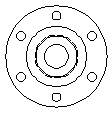
\includegraphics[scale=1]{duanguaithreeview1.png}}
\ffigbox{\caption{设置剖切线}\label{fig:duanguaithreeview3}}{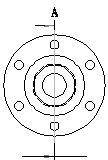
\includegraphics[scale=0.8]{duanguaithreeview3.png}}
\ffigbox{\caption{端盖视图}\label{fig:duanguaithreeview4}}{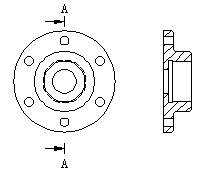
\includegraphics[scale=0.8]{duanguaithreeview4.png}}
\end{floatrow}
\end{figure}
\item 创建全剖左视图。

启动合建全剖视图的方法有:
\begin{itemize}
\item 键盘输入viewsection\index{viewsection}。
\item 【布局】$\triangleright$【截面】
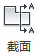
\includegraphics[scale=0.3]{viewsection.png}$\triangleright$【全剖】图标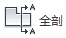
\includegraphics[scale=0.5]{quanpo.png}。
\end{itemize}
启动命令后,选择图\ref{fig:duanguaithreeview1}所示的主视图为父视图。
\begin{lstlisting}
|命令:  VIEWSECTION|
|选择父视图:找到 1 个|
\end{lstlisting}

然后,按图\ref{fig:duanguaithreeview3}所示的方式设置剖切线。
\begin{lstlisting}
|隐藏线 = 可见线 比例 = 1:2 (来自父视图)|
|指定起点或 [类型(T)/隐藏线(H)/比例(S)/可见性(V)/注释(A)/|
|图案填充(C)] $<$类型$>$:|
|指定下一个点或 [放弃(U)]: |
|指定下一个点或 [放弃(U)/完成(D)] $<$完成$>$:|
\end{lstlisting}
最后指定左视图的位置,结果如图\ref{fig:duanguaithreeview4}所示。
\begin{lstlisting}
|指定截面视图的位置或:|
|选择选项 [隐藏线(H)/比例(S)/可见性(V)/投影(P)/深度(D)/注释(A)|
|/图案填充(C)/移动(M)/退出(X)] $<$退出$>$:|
\end{lstlisting}
\end{procedure}
\endinput